\section{Zielsetzung}
\label{sec:Zielsetzung}
Das Ziel des Versuchs ist die Aufnahme und anschließende Analyse von Absorptionsspektren verschiedener Materialien und des Emissionsspektrum einer 
Kupferröntgenröhre.
\section{Theorie}
\label{sec:Theorie}
\subsection{Röntgenstrahlung}
Die Röntgenstrahlung wird in einer evakuierten Röhre dadurch erzeugt, dass durch eine anliegende Spannung beschleunigte Elektronen auf ein bestimmtes Anodenmaterial prallen. Die freien Elektronen
wurden zuvor von einer Glükathode emmitiert. Das vom Zusammenstoß stammende Röntgenspektrum kann in ein kontinuierliches Bremsspektrum und eine charakteristische 
Röntgenstrahlung unterteilt werden. \\
Das Bremsspektrum entsteht bei der Abbremsung des Elektrons im Coulombfeld der Atomkerne des Anodenmaterials. Die dadurch ausgesandten Photonen besitzen genau die 
Energie, die das Elektron durch das Abbremsen verloren hat. Das Bremsspektrum ist kontinuierlich, da ein ELektron sowohl seine gesamte kinetisch Energie auf einmal abgeben
k, als auch nur Teile davon. Die maximal mögliche Energie hängt dabei ausschließlich von der Beschleunigungsspannung ab. Das Bremsspektrum ist 
schematisch in Abbildung (\ref{fig:Bremsspektrum}) zu sehen. Die aus der maximalen Energie ableitbare minimale Wellenlänge lässt
sich durch 
\begin{equation}
    \lambda_{\text{min}} = \frac{h \cdot c}{e \cdot U}
\end{equation}
beschreiben. Dabei ist $h$ das Planksche Wirkumsquantum, $c$ die Lichtgeschwindigkeit, $e$ die Elementarladung und $U$ die angelegte Beschleunigungsspannung.\\
\begin{figure}[H]
    \centering
    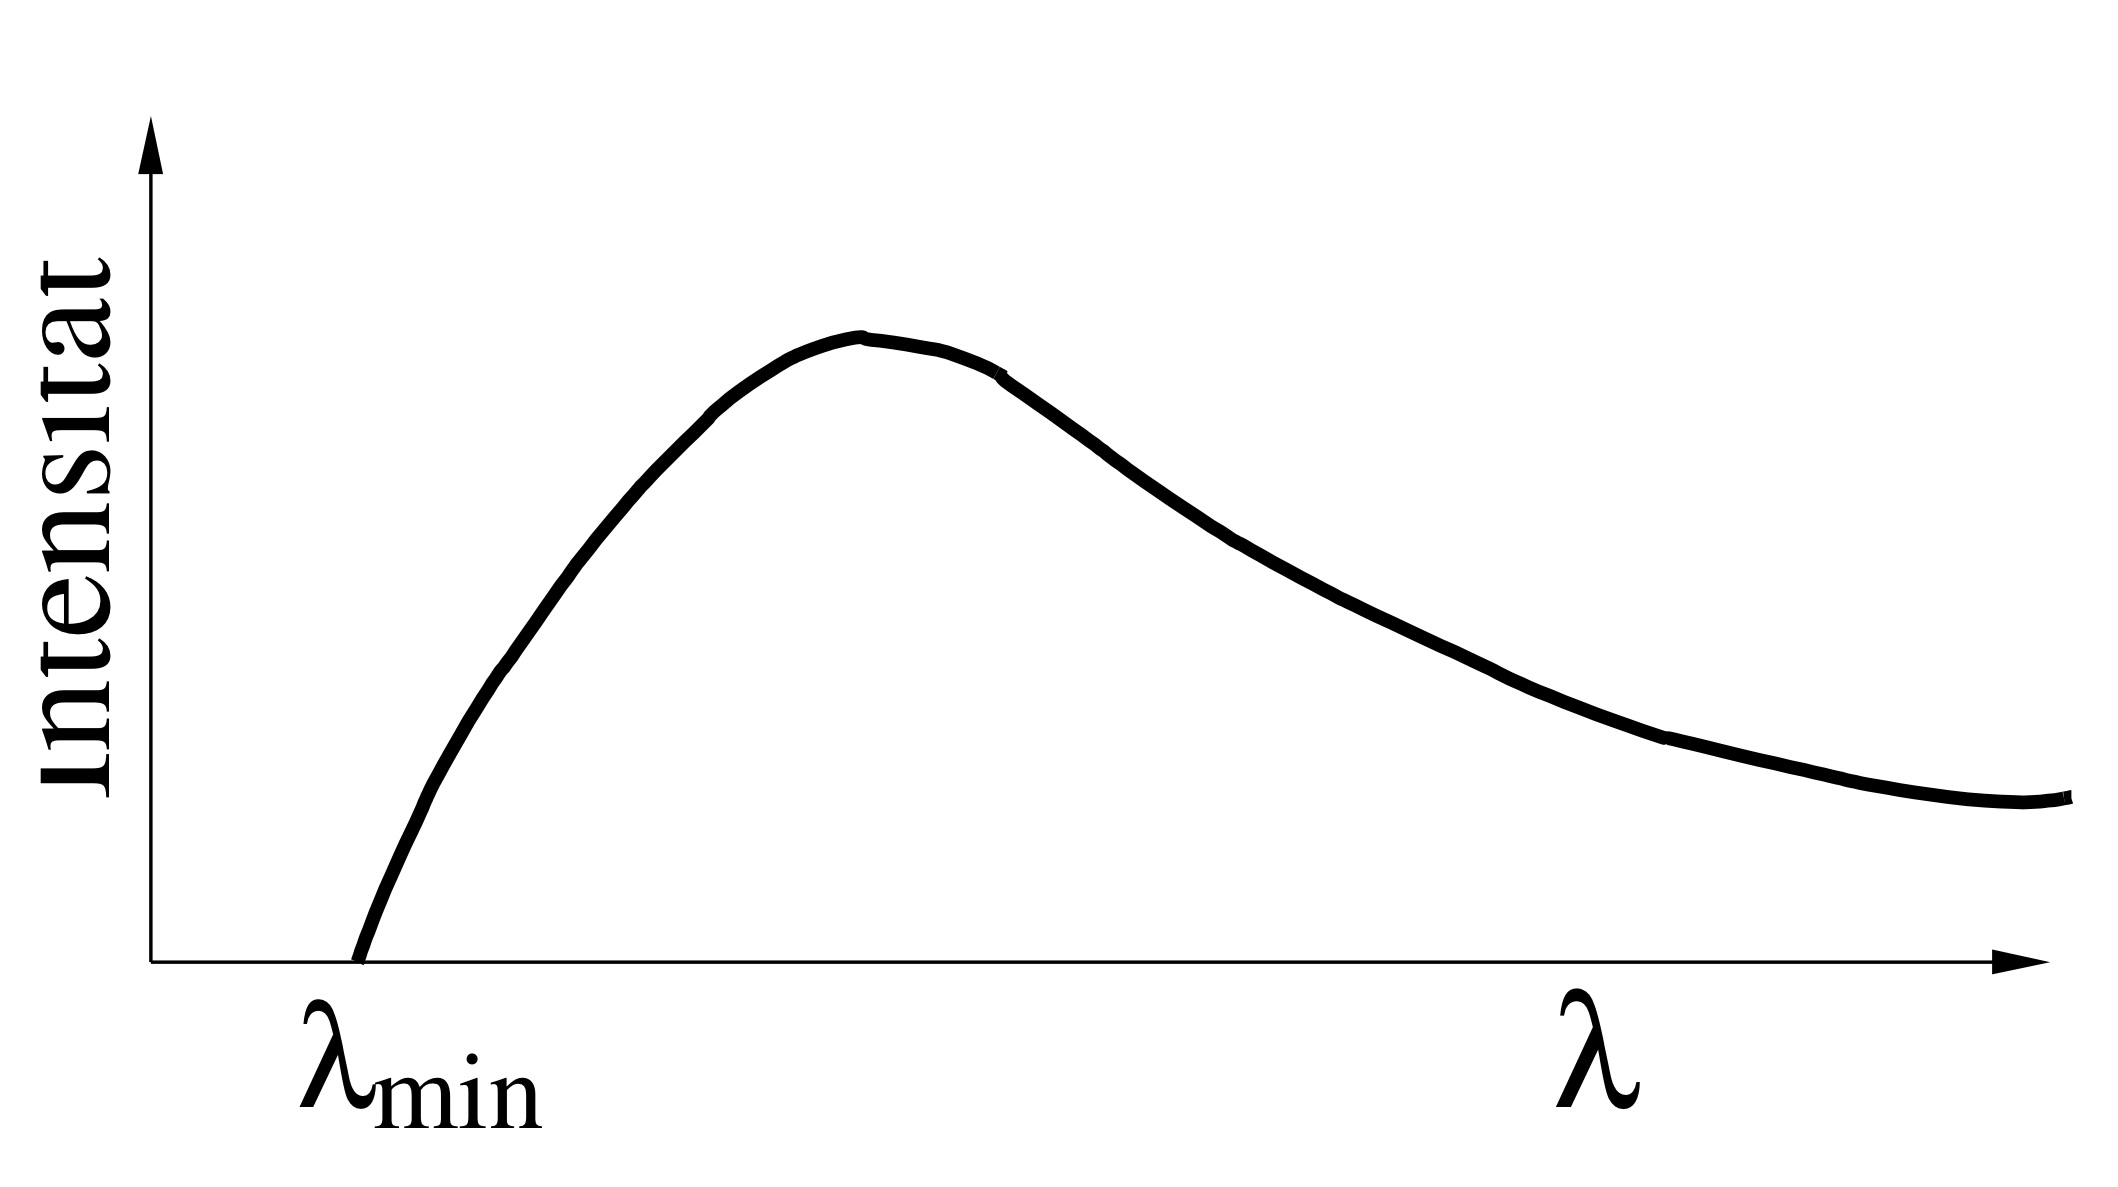
\includegraphics[width=\textwidth/2]{content/Bilder/Bremsspektrum.jpeg}
    \caption{Schematische Darstellung eines Bremsspektrums.}
    \label{fig:Bremsspektrum}
\end{figure}

Das charakteristische Röntgenspektrum ist abhängig vom Material der Anode. Es entsteht dadurch, dass das Anodenmaterial ionisiert wird, wodurch eine leere 
Elektronenschale entsteht. In diese leere Schale fällt dann ein Elektron aus einer höheren Schale herein und gibt die Energiedifferenz der Schalen als Röntgenquant 
ab. Daher besteht das charakteristische Röntgenspektrum aus scharfen Linien, die mit den Buchstaben $K_\alpha, K_\beta, L_alpha, \text{etc.}$ bezeichnet werden. Der
Großbuchstabe gibt dabei die Schale an, in die das Elektron hineinfällt und die griechischen Buchstaben geben an, aus welcher Schale es kommt. \\
Die Bindungsenergie $E_n$ der einzelnen Elektronen in der n-ten Schale kann durch die Formel 
\begin{equation}
E_n = - R_{\infty} \cdot z^{2}_{\text{eff}} \cdot \frac{1}{n²}
\end{equation}
beschrieben werden. $R_{\infty}$ ist hier die Rydbergenergie und $z_{\text{eff}}$ die effektive Kernladung, für die $z_{\text{eff}} = z - \sigma$ mit $z$ als Kernladungszahl 
und $\sigma$ als Abschirmkonstante gilt. 
Die Abschirmkonstanten können durch folgende Formen für die Energien der $\text{Cu-K}_\alpha$ - und der $\text{Cu-K}_{\beta}$ - Linie 
\begin{align}
    E_{K,\text{abs}} &= R_{\infty} \cdot \left(z - \sigma_1\right)² \label{eqn:Kupfer_Linien_Energien_abs} \\
    E_{K,\alpha} &= R_{\infty} \cdot \left(\frac{1}{n}\right)² \cdot \left(z - \sigma_1\right)² - R_{\infty} \cdot \left(\frac{1}{m}\right)² \cdot \left(z - \sigma_2\right)² \label{eqn:Kupfer_Linien_Energien_alpha}\\
    E_{K,\beta} &= R_{\infty} \cdot \left(\frac{1}{n}\right)² \cdot \left(z - \sigma_1\right)² - R_{\infty} \cdot \left(\frac{1}{l}\right)² \cdot \left(z - \sigma_3\right)² \label{eqn:Kupfer_Linien_Energien_beta}
 \end{align}
bei Vernachlässigung des Drehimpulsbeitrages berechnet werden. Für Kupfer gilt dabei $n = 1, m = 2$ und $l = 3$. \\

\subsection{Absorption von Röntgenstrahlung}
Der Compton- und der Photoeffekt sind die beiden wichtigsten Prozesse bei der Absorption von Röntgenstrahlung mit einer Energie von unter $1 \si{\mega\electronvolt}$.

\subsection{Vorbereitungsaufgaben}
\label{sec:Vorbereitungsaufgaben}
Zur Vorbereitung sollen die Energien der $\text{Cu-K}_\alpha$ - und der $\text{Cu-K}_{\beta}$ - Linie recherchiert werden. Zu diesen Energien wird der Glanzwinkel 
Theta des Briggs Kristalls mit Formel (\ref{}) bestimmt. Der Briggs Kristall ist ein LiFI Kristall mit Gitterkonstante $d = 201,4 \unit{\pico\meter}$.
Die sich ergebenden Werte sind 
\begin{align*}
    K_\alpha &= 8 \, \si{\kilo\electronvolt}\\
    \theta_\alpha &= 22,63 \unit{\degree} \\
    K_\beta &= 8,91 \, \si{\kilo\electronvolt}\\
    \theta_\beta &= 20,21 \unit{\degree} .
\end{align*}
Zusätzlich sollte die Literaturwerte der K-Kante recherchiert und die dazugehörigen Braggwinkel und Abschirmkonstanten für verschiedene Materialien berechnet werden.
Berechnet wurden die Werte mithilfe von Formel (\ref{}) und (\ref{}).
Sämtliche Werte befinden sich sortiert nach Ordnungszahl $z$ in Tabelle (\ref{tab:Vorbereitungswerte}).

\begin{table}[H]
    \centering
    \caption{Literaturwerte der K-Kante mit dazugehörigen Braggwinkel und Abschirmkonstanten verschiendener Materialien}
    \label{tab:Vorbereitungswerte}
    \begin{tblr}{colspec={l r r r r}}
        \toprule
        $\text{Material}$ & $z$ & $E^{\text{Lit}}_{\text{K}}\left[\si{\kilo\electronvolt}\right]$ & $\theta^{\text{Lit}}_{\text{K}} \left[\unit{\degree}\right]$ & $\sigma_{\text{K}}$ \\
        \midrule
        \text{Zink} & 30 & 9,65 & 18,60 & 3,56 \\
        \text{Germanium} & 32 & 11,11 & 16,09 & 3,67 \\
        \text{Brom} & 35 & 13,48 & 13,20 & 3,83 \\
        \text{Rubidium} & 37 & 15,21 & 11,68 & 3,94 \\
        \text{Strontium} & 38 & 16,12 & 11,01 & 3,98 \\
        \text{Zirconium} & 40 & 18,01 & 9,84 & 4,08 \\
        \bottomrule
    \end{tblr}
 \end{table}